% Created by tikzDevice version 0.12.3.1 on 2022-12-09 10:57:34
% !TEX encoding = UTF-8 Unicode
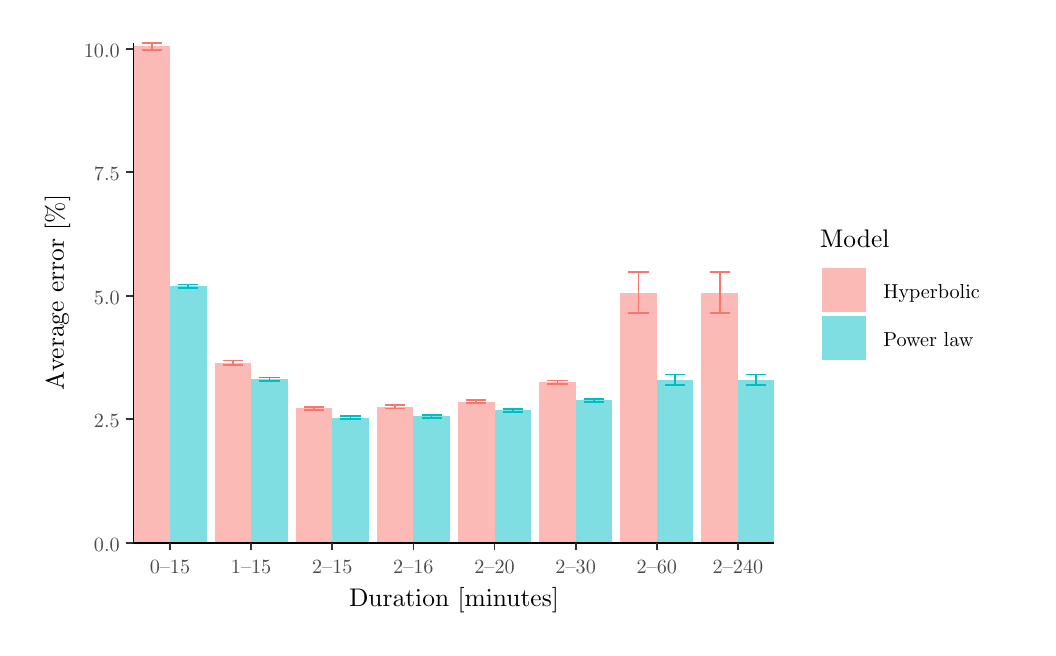
\begin{tikzpicture}[x=1pt,y=1pt]
\definecolor{fillColor}{RGB}{255,255,255}
\path[use as bounding box,fill=fillColor,fill opacity=0.00] (0,0) rectangle (361.35,216.81);
\begin{scope}
\path[clip] (  0.00,  0.00) rectangle (361.35,216.81);
\definecolor{drawColor}{RGB}{255,255,255}
\definecolor{fillColor}{RGB}{255,255,255}

\path[draw=drawColor,line width= 0.6pt,line join=round,line cap=round,fill=fillColor] (  0.00,  0.00) rectangle (361.35,216.81);
\end{scope}
\begin{scope}
\path[clip] ( 38.23, 30.69) rectangle (269.85,211.31);
\definecolor{fillColor}{RGB}{255,255,255}

\path[fill=fillColor] ( 38.23, 30.69) rectangle (269.85,211.31);
\definecolor{fillColor}{RGB}{248,118,109}

\path[fill=fillColor,fill opacity=0.50] ( 38.23, 30.69) rectangle ( 51.42,210.03);
\definecolor{fillColor}{RGB}{0,191,196}

\path[fill=fillColor,fill opacity=0.50] ( 51.42, 30.69) rectangle ( 64.62,123.40);
\definecolor{fillColor}{RGB}{248,118,109}

\path[fill=fillColor,fill opacity=0.50] ( 67.55, 30.69) rectangle ( 80.74, 95.74);
\definecolor{fillColor}{RGB}{0,191,196}

\path[fill=fillColor,fill opacity=0.50] ( 80.74, 30.69) rectangle ( 93.94, 89.80);
\definecolor{fillColor}{RGB}{248,118,109}

\path[fill=fillColor,fill opacity=0.50] ( 96.87, 30.69) rectangle (110.06, 79.21);
\definecolor{fillColor}{RGB}{0,191,196}

\path[fill=fillColor,fill opacity=0.50] (110.06, 30.69) rectangle (123.25, 75.88);
\definecolor{fillColor}{RGB}{248,118,109}

\path[fill=fillColor,fill opacity=0.50] (126.19, 30.69) rectangle (139.38, 79.75);
\definecolor{fillColor}{RGB}{0,191,196}

\path[fill=fillColor,fill opacity=0.50] (139.38, 30.69) rectangle (152.57, 76.41);
\definecolor{fillColor}{RGB}{248,118,109}

\path[fill=fillColor,fill opacity=0.50] (155.51, 30.69) rectangle (168.70, 81.70);
\definecolor{fillColor}{RGB}{0,191,196}

\path[fill=fillColor,fill opacity=0.50] (168.70, 30.69) rectangle (181.89, 78.52);
\definecolor{fillColor}{RGB}{248,118,109}

\path[fill=fillColor,fill opacity=0.50] (184.83, 30.69) rectangle (198.02, 88.62);
\definecolor{fillColor}{RGB}{0,191,196}

\path[fill=fillColor,fill opacity=0.50] (198.02, 30.69) rectangle (211.21, 82.11);
\definecolor{fillColor}{RGB}{248,118,109}

\path[fill=fillColor,fill opacity=0.50] (214.14, 30.69) rectangle (227.34,121.11);
\definecolor{fillColor}{RGB}{0,191,196}

\path[fill=fillColor,fill opacity=0.50] (227.34, 30.69) rectangle (240.53, 89.56);
\definecolor{fillColor}{RGB}{248,118,109}

\path[fill=fillColor,fill opacity=0.50] (243.46, 30.69) rectangle (256.66,121.11);
\definecolor{fillColor}{RGB}{0,191,196}

\path[fill=fillColor,fill opacity=0.50] (256.66, 30.69) rectangle (269.85, 89.56);
\definecolor{drawColor}{RGB}{248,118,109}

\path[draw=drawColor,line width= 0.6pt,line join=round] ( 41.16,211.31) --
	( 48.49,211.31);

\path[draw=drawColor,line width= 0.6pt,line join=round] ( 44.83,211.31) --
	( 44.83,208.76);

\path[draw=drawColor,line width= 0.6pt,line join=round] ( 41.16,208.76) --
	( 48.49,208.76);
\definecolor{drawColor}{RGB}{0,191,196}

\path[draw=drawColor,line width= 0.6pt,line join=round] ( 54.35,124.03) --
	( 61.68,124.03);

\path[draw=drawColor,line width= 0.6pt,line join=round] ( 58.02,124.03) --
	( 58.02,122.76);

\path[draw=drawColor,line width= 0.6pt,line join=round] ( 54.35,122.76) --
	( 61.68,122.76);
\definecolor{drawColor}{RGB}{248,118,109}

\path[draw=drawColor,line width= 0.6pt,line join=round] ( 70.48, 96.51) --
	( 77.81, 96.51);

\path[draw=drawColor,line width= 0.6pt,line join=round] ( 74.15, 96.51) --
	( 74.15, 94.97);

\path[draw=drawColor,line width= 0.6pt,line join=round] ( 70.48, 94.97) --
	( 77.81, 94.97);
\definecolor{drawColor}{RGB}{0,191,196}

\path[draw=drawColor,line width= 0.6pt,line join=round] ( 83.67, 90.38) --
	( 91.00, 90.38);

\path[draw=drawColor,line width= 0.6pt,line join=round] ( 87.34, 90.38) --
	( 87.34, 89.21);

\path[draw=drawColor,line width= 0.6pt,line join=round] ( 83.67, 89.21) --
	( 91.00, 89.21);
\definecolor{drawColor}{RGB}{248,118,109}

\path[draw=drawColor,line width= 0.6pt,line join=round] ( 99.80, 79.83) --
	(107.13, 79.83);

\path[draw=drawColor,line width= 0.6pt,line join=round] (103.46, 79.83) --
	(103.46, 78.60);

\path[draw=drawColor,line width= 0.6pt,line join=round] ( 99.80, 78.60) --
	(107.13, 78.60);
\definecolor{drawColor}{RGB}{0,191,196}

\path[draw=drawColor,line width= 0.6pt,line join=round] (112.99, 76.42) --
	(120.32, 76.42);

\path[draw=drawColor,line width= 0.6pt,line join=round] (116.66, 76.42) --
	(116.66, 75.34);

\path[draw=drawColor,line width= 0.6pt,line join=round] (112.99, 75.34) --
	(120.32, 75.34);
\definecolor{drawColor}{RGB}{248,118,109}

\path[draw=drawColor,line width= 0.6pt,line join=round] (129.12, 80.36) --
	(136.45, 80.36);

\path[draw=drawColor,line width= 0.6pt,line join=round] (132.78, 80.36) --
	(132.78, 79.14);

\path[draw=drawColor,line width= 0.6pt,line join=round] (129.12, 79.14) --
	(136.45, 79.14);
\definecolor{drawColor}{RGB}{0,191,196}

\path[draw=drawColor,line width= 0.6pt,line join=round] (142.31, 76.94) --
	(149.64, 76.94);

\path[draw=drawColor,line width= 0.6pt,line join=round] (145.98, 76.94) --
	(145.98, 75.87);

\path[draw=drawColor,line width= 0.6pt,line join=round] (142.31, 75.87) --
	(149.64, 75.87);
\definecolor{drawColor}{RGB}{248,118,109}

\path[draw=drawColor,line width= 0.6pt,line join=round] (158.44, 82.31) --
	(165.77, 82.31);

\path[draw=drawColor,line width= 0.6pt,line join=round] (162.10, 82.31) --
	(162.10, 81.08);

\path[draw=drawColor,line width= 0.6pt,line join=round] (158.44, 81.08) --
	(165.77, 81.08);
\definecolor{drawColor}{RGB}{0,191,196}

\path[draw=drawColor,line width= 0.6pt,line join=round] (171.63, 79.05) --
	(178.96, 79.05);

\path[draw=drawColor,line width= 0.6pt,line join=round] (175.30, 79.05) --
	(175.30, 77.98);

\path[draw=drawColor,line width= 0.6pt,line join=round] (171.63, 77.98) --
	(178.96, 77.98);
\definecolor{drawColor}{RGB}{248,118,109}

\path[draw=drawColor,line width= 0.6pt,line join=round] (187.76, 89.26) --
	(195.09, 89.26);

\path[draw=drawColor,line width= 0.6pt,line join=round] (191.42, 89.26) --
	(191.42, 87.98);

\path[draw=drawColor,line width= 0.6pt,line join=round] (187.76, 87.98) --
	(195.09, 87.98);
\definecolor{drawColor}{RGB}{0,191,196}

\path[draw=drawColor,line width= 0.6pt,line join=round] (200.95, 82.66) --
	(208.28, 82.66);

\path[draw=drawColor,line width= 0.6pt,line join=round] (204.62, 82.66) --
	(204.62, 81.56);

\path[draw=drawColor,line width= 0.6pt,line join=round] (200.95, 81.56) --
	(208.28, 81.56);
\definecolor{drawColor}{RGB}{248,118,109}

\path[draw=drawColor,line width= 0.6pt,line join=round] (217.08,128.48) --
	(224.41,128.48);

\path[draw=drawColor,line width= 0.6pt,line join=round] (220.74,128.48) --
	(220.74,113.75);

\path[draw=drawColor,line width= 0.6pt,line join=round] (217.08,113.75) --
	(224.41,113.75);
\definecolor{drawColor}{RGB}{0,191,196}

\path[draw=drawColor,line width= 0.6pt,line join=round] (230.27, 91.54) --
	(237.60, 91.54);

\path[draw=drawColor,line width= 0.6pt,line join=round] (233.94, 91.54) --
	(233.94, 87.58);

\path[draw=drawColor,line width= 0.6pt,line join=round] (230.27, 87.58) --
	(237.60, 87.58);
\definecolor{drawColor}{RGB}{248,118,109}

\path[draw=drawColor,line width= 0.6pt,line join=round] (246.40,128.48) --
	(253.73,128.48);

\path[draw=drawColor,line width= 0.6pt,line join=round] (250.06,128.48) --
	(250.06,113.75);

\path[draw=drawColor,line width= 0.6pt,line join=round] (246.40,113.75) --
	(253.73,113.75);
\definecolor{drawColor}{RGB}{0,191,196}

\path[draw=drawColor,line width= 0.6pt,line join=round] (259.59, 91.54) --
	(266.92, 91.54);

\path[draw=drawColor,line width= 0.6pt,line join=round] (263.25, 91.54) --
	(263.25, 87.58);

\path[draw=drawColor,line width= 0.6pt,line join=round] (259.59, 87.58) --
	(266.92, 87.58);
\end{scope}
\begin{scope}
\path[clip] (  0.00,  0.00) rectangle (361.35,216.81);
\definecolor{drawColor}{RGB}{0,0,0}

\path[draw=drawColor,line width= 0.6pt,line join=round] ( 38.23, 30.69) --
	( 38.23,211.31);
\end{scope}
\begin{scope}
\path[clip] (  0.00,  0.00) rectangle (361.35,216.81);
\definecolor{drawColor}{gray}{0.30}

\node[text=drawColor,anchor=base east,inner sep=0pt, outer sep=0pt, scale=  0.73] at ( 33.28, 27.66) {0.0};

\node[text=drawColor,anchor=base east,inner sep=0pt, outer sep=0pt, scale=  0.73] at ( 33.28, 72.28) {2.5};

\node[text=drawColor,anchor=base east,inner sep=0pt, outer sep=0pt, scale=  0.73] at ( 33.28,116.90) {5.0};

\node[text=drawColor,anchor=base east,inner sep=0pt, outer sep=0pt, scale=  0.73] at ( 33.28,161.52) {7.5};

\node[text=drawColor,anchor=base east,inner sep=0pt, outer sep=0pt, scale=  0.73] at ( 33.28,206.14) {10.0};
\end{scope}
\begin{scope}
\path[clip] (  0.00,  0.00) rectangle (361.35,216.81);
\definecolor{drawColor}{gray}{0.20}

\path[draw=drawColor,line width= 0.6pt,line join=round] ( 35.48, 30.69) --
	( 38.23, 30.69);

\path[draw=drawColor,line width= 0.6pt,line join=round] ( 35.48, 75.31) --
	( 38.23, 75.31);

\path[draw=drawColor,line width= 0.6pt,line join=round] ( 35.48,119.93) --
	( 38.23,119.93);

\path[draw=drawColor,line width= 0.6pt,line join=round] ( 35.48,164.55) --
	( 38.23,164.55);

\path[draw=drawColor,line width= 0.6pt,line join=round] ( 35.48,209.17) --
	( 38.23,209.17);
\end{scope}
\begin{scope}
\path[clip] (  0.00,  0.00) rectangle (361.35,216.81);
\definecolor{drawColor}{RGB}{0,0,0}

\path[draw=drawColor,line width= 0.6pt,line join=round] ( 38.23, 30.69) --
	(269.85, 30.69);
\end{scope}
\begin{scope}
\path[clip] (  0.00,  0.00) rectangle (361.35,216.81);
\definecolor{drawColor}{gray}{0.20}

\path[draw=drawColor,line width= 0.6pt,line join=round] ( 51.42, 27.94) --
	( 51.42, 30.69);

\path[draw=drawColor,line width= 0.6pt,line join=round] ( 80.74, 27.94) --
	( 80.74, 30.69);

\path[draw=drawColor,line width= 0.6pt,line join=round] (110.06, 27.94) --
	(110.06, 30.69);

\path[draw=drawColor,line width= 0.6pt,line join=round] (139.38, 27.94) --
	(139.38, 30.69);

\path[draw=drawColor,line width= 0.6pt,line join=round] (168.70, 27.94) --
	(168.70, 30.69);

\path[draw=drawColor,line width= 0.6pt,line join=round] (198.02, 27.94) --
	(198.02, 30.69);

\path[draw=drawColor,line width= 0.6pt,line join=round] (227.34, 27.94) --
	(227.34, 30.69);

\path[draw=drawColor,line width= 0.6pt,line join=round] (256.66, 27.94) --
	(256.66, 30.69);
\end{scope}
\begin{scope}
\path[clip] (  0.00,  0.00) rectangle (361.35,216.81);
\definecolor{drawColor}{gray}{0.30}

\node[text=drawColor,anchor=base,inner sep=0pt, outer sep=0pt, scale=  0.73] at ( 51.42, 19.68) {0--15};

\node[text=drawColor,anchor=base,inner sep=0pt, outer sep=0pt, scale=  0.73] at ( 80.74, 19.68) {1--15};

\node[text=drawColor,anchor=base,inner sep=0pt, outer sep=0pt, scale=  0.73] at (110.06, 19.68) {2--15};

\node[text=drawColor,anchor=base,inner sep=0pt, outer sep=0pt, scale=  0.73] at (139.38, 19.68) {2--16};

\node[text=drawColor,anchor=base,inner sep=0pt, outer sep=0pt, scale=  0.73] at (168.70, 19.68) {2--20};

\node[text=drawColor,anchor=base,inner sep=0pt, outer sep=0pt, scale=  0.73] at (198.02, 19.68) {2--30};

\node[text=drawColor,anchor=base,inner sep=0pt, outer sep=0pt, scale=  0.73] at (227.34, 19.68) {2--60};

\node[text=drawColor,anchor=base,inner sep=0pt, outer sep=0pt, scale=  0.73] at (256.66, 19.68) {2--240};
\end{scope}
\begin{scope}
\path[clip] (  0.00,  0.00) rectangle (361.35,216.81);
\definecolor{drawColor}{RGB}{0,0,0}

\node[text=drawColor,anchor=base,inner sep=0pt, outer sep=0pt, scale=  0.92] at (154.04,  7.64) {Duration [minutes]};
\end{scope}
\begin{scope}
\path[clip] (  0.00,  0.00) rectangle (361.35,216.81);
\definecolor{drawColor}{RGB}{0,0,0}

\node[text=drawColor,rotate= 90.00,anchor=base,inner sep=0pt, outer sep=0pt, scale=  0.92] at ( 13.08,121.00) {Average error [\%]};
\end{scope}
\begin{scope}
\path[clip] (  0.00,  0.00) rectangle (361.35,216.81);
\definecolor{fillColor}{RGB}{255,255,255}

\path[fill=fillColor] (280.85, 90.55) rectangle (355.85,151.45);
\end{scope}
\begin{scope}
\path[clip] (  0.00,  0.00) rectangle (361.35,216.81);
\definecolor{drawColor}{RGB}{0,0,0}

\node[text=drawColor,anchor=base west,inner sep=0pt, outer sep=0pt, scale=  0.92] at (286.35,137.30) {Model};
\end{scope}
\begin{scope}
\path[clip] (  0.00,  0.00) rectangle (361.35,216.81);
\definecolor{fillColor}{RGB}{248,118,109}

\path[fill=fillColor,fill opacity=0.50] (287.06,114.10) rectangle (302.98,130.02);
\end{scope}
\begin{scope}
\path[clip] (  0.00,  0.00) rectangle (361.35,216.81);
\definecolor{fillColor}{RGB}{0,191,196}

\path[fill=fillColor,fill opacity=0.50] (287.06, 96.76) rectangle (302.98,112.68);
\end{scope}
\begin{scope}
\path[clip] (  0.00,  0.00) rectangle (361.35,216.81);
\definecolor{drawColor}{RGB}{0,0,0}

\node[text=drawColor,anchor=base west,inner sep=0pt, outer sep=0pt, scale=  0.73] at (309.20,119.03) {Hyperbolic};
\end{scope}
\begin{scope}
\path[clip] (  0.00,  0.00) rectangle (361.35,216.81);
\definecolor{drawColor}{RGB}{0,0,0}

\node[text=drawColor,anchor=base west,inner sep=0pt, outer sep=0pt, scale=  0.73] at (309.20,101.69) {Power law};
\end{scope}
\end{tikzpicture}
